%%
%% This is file `sample-authordraft.tex',
%% generated with the docstrip utility.
%%
%% The original source files were:
%%
%% samples.dtx  (with options: `authordraft')
%% 
%% IMPORTANT NOTICE:
%% 
%% For the copyright see the source file.
%% 
%% Any modified versions of this file must be renamed
%% with new filenames distinct from sample-authordraft.tex.
%% 
%% For distribution of the original source see the terms
%% for copying and modification in the file samples.dtx.
%% 
%% This generated file may be distributed as long as the
%% original source files, as listed above, are part of the
%% same distribution. (The sources need not necessarily be
%% in the same archive or directory.)
%%
%%
%% Commands for TeXCount
%TC:macro \cite [option:text,text]
%TC:macro \citep [option:text,text]
%TC:macro \citet [option:text,text]
%TC:envir table 0 1
%TC:envir table* 0 1
%TC:envir tabular [ignore] word
%TC:envir displaymath 0 word
%TC:envir math 0 word
%TC:envir comment 0 0
%%
%%
%% The first command in your LaTeX source must be the \documentclass
%% command.
%%
%% For submission and review of your manuscript please change the
%% command to \documentclass[manuscript, screen, review]{acmart}.
%%
%% When submitting camera ready or to TAPS, please change the command
%% to \documentclass[sigconf]{acmart} or whichever template is required
%% for your publication.
%%
%%
\documentclass[sigconf,authordraft]{acmart}

%%
%% \BibTeX command to typeset BibTeX logo in the docs
\AtBeginDocument{%
    \providecommand\BibTeX{{%
      Bib\TeX}}}

%% Rights management information.  This information is sent to you
%% when you complete the rights form.  These commands have SAMPLE
%% values in them; it is your responsibility as an author to replace
%% the commands and values with those provided to you when you
%% complete the rights form.
%% \setcopyright{acmcopyright}
%% \copyrightyear{2023}
%% \acmYear{2023}
%% \acmDOI{XXXXXXX.XXXXXXX}

%% These commands are for a PROCEEDINGS abstract or paper.
%%\acmConference[Conference acronym 'XX]{Make sure to enter the %%correct conference title from your rights confirmation emai}{June 03--05, 2018}{Woodstock, NY}
%%
%%  Uncomment \acmBooktitle if the title of the proceedings is different
%%  from ``Proceedings of ...''!
%%
%%\acmBooktitle{Woodstock '18: ACM Symposium on Neural Gaze Detection,
%%  June 03--05, 2018, Woodstock, NY}
%%\acmPrice{15.00}
%%\acmISBN{978-1-4503-XXXX-X/18/06}


%%
%% Submission ID.
%% Use this when submitting an article to a sponsored event. You'll
%% receive a unique submission ID from the organizers
%% of the event, and this ID should be used as the parameter to this command.
%%\acmSubmissionID{123-A56-BU3}

%%
%% For managing citations, it is recommended to use bibliography
%% files in BibTeX format.
%%
%% You can then either use BibTeX with the ACM-Reference-Format style,
%% or BibLaTeX with the acmnumeric or acmauthoryear sytles, that include
%% support for advanced citation of software artefact from the
%% biblatex-software package, also separately available on CTAN.
%%
%% Look at the sample-*-biblatex.tex files for templates showcasing
%% the biblatex styles.
%%

%%
%% The majority of ACM publications use numbered citations and
%% references.  The command \citestyle{authoryear} switches to the
%% "author year" style.
%%
%% If you are preparing content for an event
%% sponsored by ACM SIGGRAPH, you must use the "author year" style of
%% citations and references.
%% Uncommenting
%% the next command will enable that style.
%%\citestyle{acmauthoryear}


%%
%% end of the preamble, start of the body of the document source.
\begin{document}

%%
%% The "title" command has an optional parameter,
%% allowing the author to define a "short title" to be used in page headers.
\title{From Synthesis to Realism: Enhancing Logistics with Computer Vision and Domain-Adversarial Training}

%%
%% The "author" command and its associated commands are used to define
%% the authors and their affiliations.
%% Of note is the shared affiliation of the first two authors, and the
%% "authornote" and "authornotemark" commands
%% used to denote shared contribution to the research.


\author{Quoc-Cuong Dang}
\affiliation{%
\institution{Ha Noi University of Science and Technology}
}
\email{cuong.dq204902@sis.hust.edu.vn}

\author{Trung-Dung Nguyen}
\affiliation{%
\institution{Ha Noi University of Science and Technology}
}
\email{dung.nt204906@sis.hust.edu.vn}

\author{Ha-Dat Mai}
\affiliation{%
  \institution{Ha Noi University of Science and Technology}
}
\email{dat.mh200135@sis.hust.edu.vn}

\author{Van-Duc Vu}
\affiliation{%
\institution{FPT University}
}
\email{ducvvhe176438@fpt.edu.vn}

\author{Ngoc-Anh Hoang}
\affiliation{%
\institution{FPT University}
}
\email{anhhnhe186401@fpt.edu.vn}

\author{Thu-Uyen Nguyen}
\affiliation{%
\institution{FPT University}
}
\email{uyennthe176614@fpt.edu.vn}

\author{Van-Thiep Nguyen}
\affiliation{%
\institution{FPT University}
}
\email{thiepnvhe173027@fpt.edu.vn}

\author{Phan Xuan Tan}
\affiliation{%
\institution{Shibaura Institute of Technology}
}
\email{tanpx@shibaura-it.ac.jp}

\author{Phong-Tung Doan
(Corresponding author)}
\affiliation{%
\institution{Ha Noi University of Science and Technology}
}
\email{tungdp@soict.hust.edu.vn}


\author{Dinh-Cuong Hoang}
\affiliation{%
\institution{FPT University}
}
\email{cuonghd12@fe.edu.vn}

%%
%% By default, the full list of authors will be used in the page
%% headers. Often, this list is too long, and will overlap
%% other information printed in the page headers. This command allows
%% the author to define a more concise list
%% of authors' names for this purpose.
%% \renewcommand{\shortauthors}{.}

%%
%% The abstract is a short summary of the work to be presented in the
%% article.
\begin{abstract}
    In the dynamic landscape of industrial logistics, the precise identification of pallet locations is pivotal for efficient supply chain operations. Leveraging recent advancements in computer vision and the affordability of cameras, our research addresses the challenge of automated pallet detection in factory settings. We propose an innovative approach that combines synthetic data generation with domain adaptation techniques. The integration of synthetic and real-world unlabeled data, guided by domain adversarial training, overcomes challenges related to data scarcity and domain shift. Experiments demonstrate the effectiveness of our approach in classifying pallet states. The results showcase the model's adaptability to real-world variations, achieving impressive accuracy. Our work not only optimizes resource allocation in warehouses but also offers a blueprint for the seamless integration of Computer Vision into broader logistics applications. The transformative potential of our methodology is underscored by its efficiency, autonomy, and applicability across industries reliant on robust supply chain management.
\end{abstract}

%%
%% The code below is generated by the tool at http://dl.acm.org/ccs.cfm.
%% Please copy and paste the code instead of the example below.
%%
\begin{CCSXML}
<ccs2012>
   <concept>
       <concept_id>10010147.10010178.10010224.10010245.10010251</concept_id>
       <concept_desc>Computing methodologies~Object recognition</concept_desc>
       <concept_significance>100</concept_significance>
       </concept>
   <concept>
       <concept_id>10010147.10010257.10010293.10010294</concept_id>
       <concept_desc>Computing methodologies~Neural networks</concept_desc>
       <concept_significance>300</concept_significance>
       </concept>
   <concept>
       <concept_id>10010147.10010178.10010224</concept_id>
       <concept_desc>Computing methodologies~Computer vision</concept_desc>
       <concept_significance>500</concept_significance>
       </concept>
   <concept>
       <concept_id>10010147.10010257.10010282.10011305</concept_id>
       <concept_desc>Computing methodologies~Semi-supervised learning settings</concept_desc>
       <concept_significance>100</concept_significance>
       </concept>
 </ccs2012>
\end{CCSXML}

\ccsdesc[100]{Computing methodologies~Object recognition}
\ccsdesc[300]{Computing methodologies~Neural networks}
\ccsdesc[500]{Computing methodologies~Computer vision}
\ccsdesc[100]{Computing methodologies~Semi-supervised learning settings}

%%
%% Keywords. The author(s) should pick words that accurately describe
%% the work being presented. Separate the keywords with commas.
\keywords{Domain Adaptation, Synthetic Data, DANN, Pallet Recognition, Pallet Dataset Creating}
%% A "teaser" image appears between the author and affiliation
%% information and the body of the document, and typically spans the
%% page.

%%\received{20 February 2007}
%%\received[revised]{12 March 2009}
%%\received[accepted]{5 June 2009}

%%
%% This command processes the author and affiliation and title
%% information and builds the first part of the formatted document.
\maketitle

\section{Introduction}
In today's dynamic industrial landscape, logistics plays a pivotal role in ensuring smooth supply chain operations by orchestrating the seamless flow of goods from origin to destination. Fundamental tasks such as stacking, unloading, and intra-warehouse movements are essential in this process, with the precise identification of pallet locations being of utmost importance. Recent technological advancements, including the widespread availability of cost-effective cameras and the successful implementation of computer vision, have revolutionized logistics operations\cite{21,22, hoang2019object, hoang2020object, vu2024occlusion, palleschi2020fully}. The affordability of cameras has led to their widespread adoption in warehouses and distribution centers, while computer vision has enabled accurate identification and tracking of objects\cite{26, 27, 28, hoang2016sub, hoang2022context, hoang2023grasp, hoang2022voting}, particularly pallets, within the logistics environment.

\noindent However, as the industry increasingly explores the potential of Computer Vision for automated pallet detection in factory settings, a significant hurdle emerges the need for substantial real-world labeled data, presenting challenges in terms of both time and cost for data labeling. Some have turned to synthetic data generation as a solution\cite{1}\cite{2}\cite{3}, but this approach encounters its obstacle known as domain shift.

\noindent To tackle these challenges, we propose an innovative approach that combines synthetic data for training with domain adaptation techniques. We utilize Blender, an open-source 3D creation suite, for generating images and labels, and incorporate Domain-Adversarial Training of Neural Networks\cite{4}. Our methodology comprises three key components: a pre-trained ResNet-34\cite{6} serving as the feature extractor, a class classifier, and a domain classifier. The distinctive feature of this architecture lies in the domain classifier, which plays a crucial role in enhancing the model's domain adaptation capabilities. Importantly, the implementation of the Domain-Adversarial Training of Neural Networks method necessitates a significant amount of real-world unlabeled data.

\noindent Building upon our methodology, we proceeded to conduct experiments to validate its effectiveness in a classification task, specifically discerning whether an image depicts an absence of a pallet, an empty pallet, or a pallet laden with goods. This classification holds significant operational implications. In cases where no pallet is detected, intervention is kept to a minimum. If only a pallet is identified, a smaller lifting device suffices. However, when goods are present on the pallet, a larger lifting device becomes imperative. Mastering this classification task promises substantial advantages in optimizing resource allocation within the warehouse.

\noindent The training phase involved an iterative process, wherein the synthetic data generated through Blender was seamlessly integrated with a carefully curated subset of real-world unlabeled data. This fusion of synthetic and real data not only addressed the scarcity of labeled samples but also facilitated the adaptation of the model to the specific nuances of the factory setting. The Domain-Adversarial Training of Neural Networks (DANN) technique played a pivotal role in bridging the gap between synthetic and real-world domains

\noindent The experimental results unequivocally showcase that the suggested approach delivers impressive performance and bears great potential for far-reaching applications within the field of automated logistics. Through the strategic integration of Deep Learning alongside domain adaptation techniques, we not only augment the effectiveness of existing operations but also lay the foundation for future breakthroughs in autonomous logistics systems.
\begin{figure*}
  \centering
  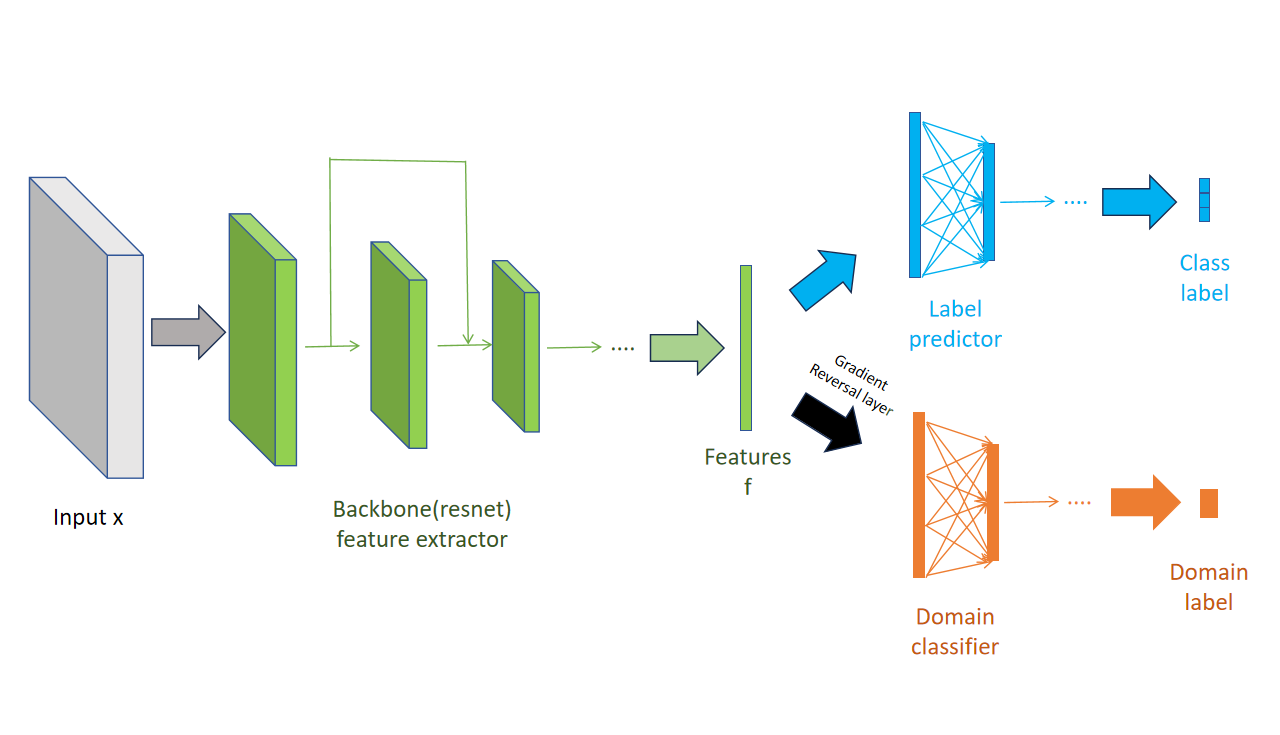
\includegraphics[width=1\textwidth]{images/model.png}
  \caption{Model structure. The model contains 3 main components: The backbone block, the class predictor block, the domain classifier block.}
  \label{fig:your-image}
\end{figure*}
\noindent In summary, our research marks a substantial leap forward in addressing crucial challenges related to automated pallet detection in factory settings, concurrently optimizing financial resources for labeling data. Through the integration of synthetic data generation and domain adaptation, we've established a robust methodology that produces precise and dependable outcomes without the need for actual labeled data. This not only streamlines the effort, time, and financial investments typically associated with labeling data but also guarantees consistently positive results. The significance of this work transcends the warehouse, providing a comprehensive blueprint for the seamless integration of Computer Vision techniques into the broader logistics landscape.

\section{Related works}
\noindent\textbf{Image Classification}

\noindent
The evolution of image classification, a fundamental task in computer vision with applications from medical diagnosis to autonomous vehicles\cite{23}, has seen a significant shift in methodologies, datasets, and performance metrics over the years. Initial approaches to image classification relied heavily on handcrafted features and traditional machine learning algorithms, such as Histogram of Oriented Gradients (HOG)\cite{5} and Scale-Invariant Feature Transform (SIFT) combined with classifiers like Support Vector Machines (SVM). While these methods showed promising results on certain tasks, they struggled with complex and diverse datasets. The landscape changed with the introduction of Convolutional Neural Networks (CNNs), with LeNet-5 being a pioneering example. Further advancements were seen with AlexNet\cite{7}, VGGNet\cite{8}, and GoogLeNet\cite{9}, which exhibited deeper architectures that significantly improved classification accuracy by extracting hierarchical features.

\noindent 
To combat the challenges of limited labeled data, the strategy of transfer learning and fine-tuning became prevalent. This involved using models pre-trained on extensive datasets like ImageNet\cite{15} and fine-tuning them for specific tasks, leading to improved generalization capabilities and resource efficiency\cite{24}. Attention mechanisms, particularly Self-Attention in Transformer models\cite{12}, also gained prominence, enabling models to focus on relevant image regions and enhancing the discriminative power of image representations. The field also saw an increased focus on adversarial defense and robustness, with techniques like adversarial training\cite{25} and robust optimization aimed at tackling the vulnerability of image classification models to adversarial attacks.

\noindent 
The progression of image classification has been significantly shaped by the accessibility of extensive datasets like ImageNet, CIFAR-10, and COCO, which have become pivotal benchmarks for evaluating and comparing models. In assessing model performance, the field has moved beyond traditional accuracy metrics to embrace a diverse range of measures, including precision, recall, F1 score, and AUC-ROC. Our research incorporates some of these metrics to comprehensively evaluate the efficiency of our model. This shift in evaluation methods mirrors the broader transition from handcrafted features to advanced deep learning architectures. The continuous exploration of novel approaches underscores a commitment to pushing the limits of image classification performance, necessitating a nuanced understanding beyond basic accuracy metrics.

\noindent\textbf{Domain Adaptation}

\noindent Domain Adaptation is a machine learning and data science technique aimed at addressing a common challenge: when the distribution of data in the source domain, where a model is trained, differs from the distribution of data in the target domain, where the model is deployed or tested. In other words, it deals with situations where the model may not perform well on new, unseen data due to differences between the training and test data distributions.

\noindent Domain adaptation aims to bridge this gap by making the model more robust to domain shifts. It involves techniques that help the model generalize better to the target domain despite being trained on a different source domain.

\noindent Key concepts and methods in domain adaptation include:

\textbf{Feature Adaptation:} Modifying the input features to make them more domain-invariant. This can involve various techniques like feature selection, dimensionality reduction, or feature transformation.\cite{16}

\textbf{Instance Re-weighting:} Giving different weights to instances from the source and target domains during training to reduce the impact of the domain shift.

\textbf{Model Adaptation:} Adjusting the model parameters to account for domain differences. Methods such as domain adversarial training or fine-tuning are often used.\cite{17}

\textbf{Transfer Learning:} Utilizing knowledge learned from the source domain to improve performance on the target domain. This can include pre-trained models or shared representations.\cite{18}

\textbf{Domain Shift Detection:} Identifying when a domain shift occurs and adapting the model accordingly. Statistical tests and anomaly detection methods can be applied.

\noindent Domain adaptation is valuable in various real-world scenarios, such as sentiment analysis, image classification, and speech recognition, where the source and target domains may exhibit differences in terms of data distribution, data collection settings, or domain-specific factors. It plays a crucial role in ensuring that machine learning models perform effectively when deployed in practical applications where data can vary significantly.

\noindent\textbf{Domain-Adversarial Training of Neural Networks}

\noindent Top-performing deep architectures are trained on massive amounts of labeled data. In the absence of labeled data for a certain task, domain adaptation often provides an easy-to-get and cheap option given that labeled data of similar nature but from a different domain (e.g. synthetic images) are available. The Domain-Adversarial Training of Neural Networks paper proposed a new approach to domain adaptation in deep architectures known as DANN that can be trained on large amounts of labeled data from the source domain and large amounts of unlabeled data from the target domain (no labeled target domain data is necessary). As the training progresses, the approach promotes the emergence of “deep” features that are discriminate for the main learning task on the source domain and invariant with respect to the shift between the domains. The authors show that this adaptation behaviour can be achieved in almost any feed-forward model by augmenting it with a few standard layers and a simple new gradient reversal layer. The resulting augmented architecture can be trained using standard back-propagation. Overall, the approach can be implemented with little effort using any of the deep-learning packages. The method performs very well in a series of image classification experiments, achieving an adaptation effect in the presence of big domain shifts and outperforming previous state-of-art on Office datasets. 

\noindent The paper Incremental Unsupervised Domain-Adversarial Training of Neural Networks\cite{19}  focuses on incremental domain adaptation, where the model is adapted iteratively to the new domain by adding selected target samples to the source training set. This approach outperforms other state-of-the-art DA algorithms in various datasets. The paper makes use of DANN structure to identify the target samples on which there is greater confidence about their true label. The output of the model is analyzed in different ways to determine the candidate samples. The selected samples are then added to the source training set by self-labeling, and the process is repeated until all target samples are labeled. This approach implements a form of adversarial training in which, by moving the self-labeled samples from the target to the source set, the DA algorithm is forced to look for new features after each iteration.
\noindent

\section{Methodology}
\subsection{Model Building Overview}
Building upon the successful domain-adversarial training framework (DANN), our approach tailors this architecture specifically for image classification tasks. We introduce targeted modifications to the DANN structure to effectively address the unique challenges and requirements of image classification. By leveraging the strengths of DANN while incorporating domain-specific adaptations, we aim to achieve superior performance in adapting models to new image classification domains. The model structure is presented in Figure 1.

\noindent In Figure 1, the employed model comprises key components: a backbone feature extractor, a layer for predicting labels, and a domain classifier layer integrated with a preceding gradient reversal layer. During each batch iteration, both real and synthetic data are fed into the model. This, coupled with the incorporation of a gradient reversal layer prior to the domain classifier, constitutes our adversarial training approach.
\subsection{Backbone}
ResNet is a convolution neural network (CNN) architecture for image classification. It was first introduced in the paper "Deep Residual Learning for Image Recognition" by He et al. (2016)\cite{20} and has since become one of the most popular CNN architectures for a variety of tasks. The backbone we proposed for the model is pretrained ResNet-34. ResNet-34 consists of 34 convolutional layers, with each layer followed by a batch normalization layer and a ReLU activation function. The network also includes four "shortcut connections" that bypass groups of convolutional layers which are called residual blocks which are illustrated in Figure 2, the shortcut connection prevents vanishing gradients, enabling the network to learn long-range dependencies and deeper representations. These shortcut connections help to alleviate the vanishing gradient problem and allow the network to learn deeper representations. 
\subsection{Domain classifier and Label Predictor}
\noindent Assume input is in m-dimensional real vector space, we have the space of the input \(x = R^m\). Let \(F_e(x, \theta_e)\) be the features map we get from the backbone. Also, we denote the label predictor layer and domain classifier layer output as \(F_l(x, \theta_l)\) and \(F_d(x, \theta_d)\) correspondingly. In the 3-layer output above, x is the input, with \(\theta_e, \theta_l, \theta_d\) as the parameters of the corresponding layer. With \(y_i\) as the ground truth of the data point \(x_i\), \(L_l()\) as the loss function, we denoted the loss function for label and domain head:
\begin{equation}
  L_l^i(\theta_e, \theta_l) = L_l(F_l(F_e(x_i, \theta_e), \theta_l), y_i)
\end{equation}
\begin{equation}
  L_d^i(\theta_e, \theta_d) = L_l(F_d(F_e(x_i, \theta_e), \theta_d), d_i)
\end{equation}
\noindent To achieve adversarial training between the domain classifier and label predictor, we employ a reverse layer that inverts the gradient descent process from the domain classifier head by negating the calculated gradient. Subsequently, we train the model on both target and source data, but only the domain loss is calculated on the target data cause we assume the lack of labeled target data, as outlined in equation (3). This negative gradient descent from the domain head, coupled with losses from both source and target domains, is designed to prevent the model from discriminating between data originating from different domains. Consequently, the target domain label classifier is effectively trained using only labeled source data (synthetic data).
\subsection{Data Feeding Mechanism}
\noindent For each batch in an epoch, we will consecutively iterate through both the source dataset and target dataset, each will be denoted as S and T, respectively. For each iteration, the input data into the model will be \(X^S_i\) and \(X^T_i\). After forwarding both data batches through the model, we will calculate the domain and label losses for both input data batches, and get \(Ls_l^i, Ls_d^i, Lt_d^i\). We don't get label loss for the target data for archiving the tasks of training data image classification of target domain data with only labeled source(synthetic) domain data.
The main Loss we use will be:
\begin{equation}
  L_i = \lambda_1.Ls_l^i + \lambda_2.Ls_d^i + \lambda_3.Lt_d^i
\end{equation}

\noindent With each \(\lambda\) as the coefficients, we can experiment and choose the appropriate proportion of each loss. Also, the loss we use will be Cross-Entropy loss:
\begin{equation}
    Loss = -\sum_{c=0}^{N-1} y_{i, c}.\log(p_{i, c})
\end{equation}
With \(N\) is the number of classes, \(y\)- binary indicator (0 or 1) if class label \(c\) is the correct classification for observation  \(i\), \(p\) is predicted probability observation \(i\) is of class \(c\).

\begin{figure}[h]
  \centering
  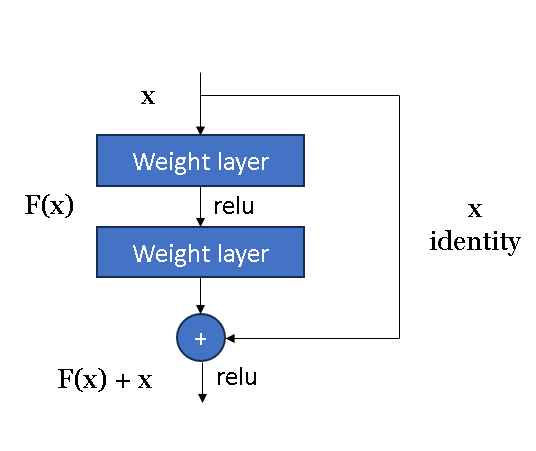
\includegraphics[width=0.48\textwidth]{images/res_block.png}
  \caption{The residual block structure.}
  \label{fig:your-image}
\end{figure}


\section{Experimental Setup}

\subsection{Dataset}
Regarding our dataset, we have meticulously annotated both real and synthetic images related to pallets. The dataset comprises three distinct labels: "No pallet" "Pallet only" and "Goods on pallet". The label "No pallet" indicates the absence of a pallet in the image, suggesting either the presence of goods or an empty scene. "Pallet only" signifies the presence of a pallet in the image, without any accompanying goods. On the other hand, "Goods on pallet" denotes the presence of goods positioned on the pallet.

\noindent Our synthetic dataset, meticulously crafted using Blender, an open-source and versatile 3D graphics software, caters to diverse applications such as animation, visual effects, 3D printing, and video game development. Our focus lies in designing warehouse scenes within Blender, featuring key elements like pallets, goods, forklifts, and containers. To ensure comprehensive coverage, we implement camera movements and automate scene capture, yielding 1000 images per scene. Simultaneously, our Python scripting integrated into Blender handles automated labeling, encompassing tasks such as image classification, object detection, segmentation, and pose estimation. This automation taps into accurate object coordinates and orientations extracted from Blender, showcasing the software's adaptability.

\noindent Moreover, Blender's flexibility allows us to experiment with various lighting conditions, augmenting dataset diversity. Each image in our dataset is standardized to a size of (480,480), and the total number of images stands at an impressive 12,000, distributed evenly with 4000 images for each class.

\noindent The advantages of our automated labeling approach are particularly prominent in terms of time and cost efficiency, providing a viable alternative to the traditionally labor-intensive process of manually labeling real-world data for intricate computer vision tasks. Synthesizing datasets through Blender's 3D graphics and Python scripting not only streamlines image classification training but also emerges as a cost-effective and time-efficient solution for advanced computer vision applications.

\noindent Moving beyond image classification, our synthetic dataset creation process has successfully delved into object detection, a traditionally time-consuming task prone to manual errors. Leveraging Blender's 3D environment and Python scripting, we efficiently extract and incorporate precise object coordinates and types into the automated labeling process. This successful application in object detection underscores the versatility and effectiveness of our synthetic dataset generation approach, demonstrating its capacity to address complex computer vision tasks that typically demand substantial time and effort for manual labeling.

\noindent Regarding our dataset of real images, we have captured pallet-related videos with all three labels. For the labels "no pallet" and "goods on pallets," we have included various types of goods on the pallet to ensure dataset generalization. These videos are recorded at a resolution of 1440x1440 pixels, featuring a square image shape that facilitates the cropping data preprocessing step, making it both easier and more precise. The videos we've captured are recorded at 60 frames per second, with each video having a duration of approximately 50-60 seconds. However, we will not be including all frames in our dataset due to the high similarity of some frames, resulting from minor changes in pallet angles during recording. Therefore, for each label, we will select only approximately 1000 images. An illustrative example of our two datasets is shown in Figure 3.


\begin{figure}[h]
  \centering
  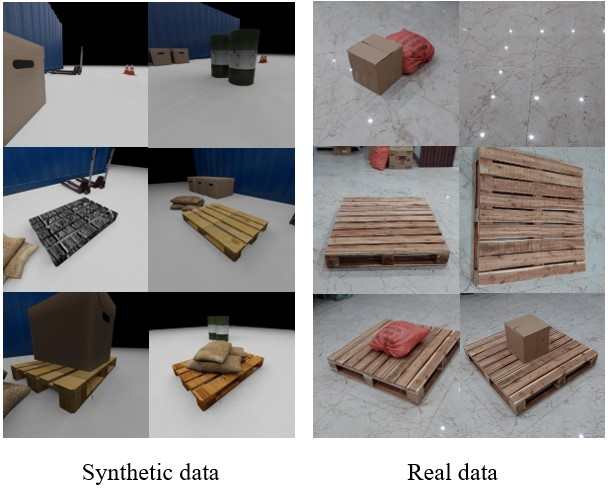
\includegraphics[width=0.48\textwidth]{images/dataset.jpg}
  \caption{The gallery of our synthetic and real datasets.}
  \label{fig:your-image}
\end{figure}

\subsection{Setup}
In this experimental study, we conducted a 30-epoch training using the Adam optimizer and ResNet34 pretrained on ImageNet1K. The final layer of the ResNet34 backbone generated a 512-dimensional latent representation, enriching the model's feature space. With a batch size of 16 and an initial learning rate of 0.001, we meticulously preprocessed input images by resizing them to (256,256) and applying a random crop to ensure standardization at (224,224). The model architecture, consisting of class and domain classifiers, incorporated a Fully Connected layer, ReLU activation function, and Dropout layer, fostering the learning of hierarchical representations. Post-training, a thorough evaluation of the model's performance informed hyperparameter fine-tuning, while data augmentation techniques were introduced to fortify the model's resilience. Our exploration included transfer learning strategies, fine-tuning for domain-specific challenges, and iterative adjustments to achieve optimal results. Simultaneously, rigorous testing on independent datasets verified the model's generalization and practical utility, concluding a systematic and refined approach to model development.

\subsection{Experimental results}
\noindent
\begin{table*}
  \caption{Score of our models}
  \label{table Score of our models}
  \begin{tabular}{c|cccc}
    \toprule
    Method&F1 score&Precision&Recall&Accuracy\\
    \midrule
     Ours(train by synthetic, without DANN)&0.81&0.85&0.77&0.79\\
     Ours(train by real, without DANN)&1&1&1&1\\
     Ours(DANN without augmentation)&0.77&0.78&0.75&0.76\\ 
     Ours(DANN, ResNet-18)&0.84&0.85&0.82&0.84\\
     Ours(DANN, ResNet-34)&0.99&0.99&0.99&0.99\\
  \bottomrule
\end{tabular}
\end{table*}
Data Augmentation Strategies:
During our experimentation, we explored several data augmentation strategies, including mosaic, cutmix, mixup, and simpler techniques like image flipping and rotation. The results revealed that the complex augmentation techniques, such as mosaic, cutmix, and mixup, did not yield significant benefits and, in some instances, led to a reduction in performance. With preprocessing techniques in this section, we delve into the systematic examination of preprocessing techniques applied to our automated pallet classification model. The insights garnered from this analysis are pivotal in understanding the influence of preprocessing on the model's performance. The application of preprocessing techniques significantly influenced the model's performance. The normalization step, is implemented through transforms.Normalize(mean=(0.485, 0.456, 0.406), std=(0.229, 0.224, 0.225)), and the use of transforms.Ran- domCrop(224) played a pivotal role in surpassing the 0.9 accuracy threshold. Normalizing input images helped the model better adapt to variations in lighting conditions and color distributions, leading to improved overall performance. Employing random cropping at the size of 224x224 pixels contributed to spatial feature extraction, enhancing the model's ability to discern critical details.
Model Sensitivity: Comparing different backbone architectures, we observed that ResNet34 consistently outperformed ResNet18 in terms of accuracy. The deeper architecture of ResNet34 provided a more expressive feature representation, enabling the model to capture intricate details and patterns more effectively. This finding emphasizes the importance of selecting a suitable backbone architecture tailored to the complexity of the classification task.
The experiment "Train by synthetic, without DANN" illustrated the model's transferability from synthetic to real data, achieving stable performance on the test set. In contrast, "Train=real, without DANN" demonstrated that the model reached maximum accuracy when trained and tested on the same real-world data source. The results of "DANN without augmentation" and "DANN, ResNet-18" continued to emphasize the role of DANN in reducing the domain gap between the two data domains. Ultimately, Ours yielded the most impressive performance, with metrics approaching their maximum values. The flexible integration of augmentation, DANN, and the ResNet-34 model architecture produced a robust model, showcasing the transferability and effectiveness of the proposed method in the real-world pallet classification task.
The experimental results underscore the effectiveness of our proposed methodology in tackling the automated pallet detection challenge. On the source dataset, our model achieved an outstanding accuracy of 0.99, showcasing its capability to accurately classify pallet states within a controlled environment.
Moreover, on the target dataset, our model demonstrated a commendable accuracy of 0.99. This performance on the target dataset signifies the success of our domain adaptation techniques in ensuring the model's adaptability to real-world variations and shifts in data distribution. The summary of our results is written in Table 1: Score of our models
\section{Conclusion}
\noindent
In conclusion, our research presents a pioneering solution to the automated pallet detection challenge within factory settings. By synergizing synthetic data generation through Blender with domain adaptation techniques, we have established a robust methodology capable of delivering accurate and reliable results. This integrated approach not only addresses the scarcity of labeled samples but also facilitates model adaptation to the nuanced realities of factory environments.
The potential impact of our work extends beyond warehouse confines, offering a comprehensive blueprint for seamlessly integrating Computer Vision techniques into the broader logistics landscape. As we envision the future of autonomous logistics systems, our proposed methodology stands as a testament to the transformative power of combining cutting-edge technologies for real-world problem-solving. The success of our approach signifies a promising direction for enhancing the efficiency and autonomy of logistics operations, with implications for diverse industries reliant on seamless supply chain management.




%%
%% The acknowledgments section is defined using the "acks" environment
%% (and NOT an unnumbered section). This ensures the proper
%% identification of the section in the article metadata, and the
%% consistent spelling of the heading.
\begin{acks}
To Robert, for the bagels and explaining CMYK and color spaces.
\end{acks}

%%
%% The next two lines define the bibliography style to be used, and
%% the bibliography file.
\bibliographystyle{ACM-Reference-Format}
\bibliography{sample-base}


%%
%% If your work has an appendix, this is the place to put it.
\appendix


\end{document}
\endinput
%%
%% End of file `sample-authordraft.tex'.
